
%%%%%%%%%%%%%%%%%%%%%%%%%%%%%%%%%%%%%%%%%%%%%%%%%%%%%%%%%%%%%%%%%%%%%
%% This is a (brief) model paper using the achemso class
%% The document class accepts keyval options, which should include
%% the target journal and optionally the manuscript type.
%%%%%%%%%%%%%%%%%%%%%%%%%%%%%%%%%%%%%%%%%%%%%%%%%%%%%%%%%%%%%%%%%%%%%
\documentclass[journal=jacsat,manuscript=article]{achemso}

%%%%%%%%%%%%%%%%%%%%%%%%%%%%%%%%%%%%%%%%%%%%%%%%%%%%%%%%%%%%%%%%%%%%%
%% Place any additional packages needed here.  Only include packages
%% which are essential, to avoid problems later. Do NOT use any
%% packages which require e-TeX (for example etoolbox): the e-TeX
%% extensions are not currently available on the ACS conversion
%% servers.
%%%%%%%%%%%%%%%%%%%%%%%%%%%%%%%%%%%%%%%%%%%%%%%%%%%%%%%%%%%%%%%%%%%%%
\usepackage[version=3]{mhchem} % Formula subscripts using \ce{}

%%%%%%%%%%%%%%%%%%%%%%%%%%%%%%%%%%%%%%%%%%%%%%%%%%%%%%%%%%%%%%%%%%%%%
%% If issues arise when submitting your manuscript, you may want to
%% un-comment the next line.  This provides information on the
%% version of every file you have used.
%%%%%%%%%%%%%%%%%%%%%%%%%%%%%%%%%%%%%%%%%%%%%%%%%%%%%%%%%%%%%%%%%%%%%
%%\listfiles

%%%%%%%%%%%%%%%%%%%%%%%%%%%%%%%%%%%%%%%%%%%%%%%%%%%%%%%%%%%%%%%%%%%%%
%% Place any additional macros here.  Please use \newcommand* where
%% possible, and avoid layout-changing macros (which are not used
%% when typesetting).
%%%%%%%%%%%%%%%%%%%%%%%%%%%%%%%%%%%%%%%%%%%%%%%%%%%%%%%%%%%%%%%%%%%%%
\newcommand*\mycommand[1]{\texttt{\emph{#1}}}

%%%%%%%%%%%%%%%%%%%%%%%%%%%%%%%%%%%%%%%%%%%%%%%%%%%%%%%%%%%%%%%%%%%%%
%% Meta-data block
%% ---------------
%% Each author should be given as a separate \author command.
%%
%% Corresponding authors should have an e-mail given after the author
%% name as an \email command. Phone and fax numbers can be given
%% using \phone and \fax, respectively; this information is optional.
%%
%% The affiliation of authors is given after the authors; each
%% \affiliation command applies to all preceding authors not already
%% assigned an affiliation.
%%
%% The affiliation takes an option argument for the short name.  This
%% will typically be something like "University of Somewhere".
%%
%% The \altaffiliation macro should be used for new address, etc.
%% On the other hand, \alsoaffiliation is used on a per author basis
%% when authors are associated with multiple institutions.
%%%%%%%%%%%%%%%%%%%%%%%%%%%%%%%%%%%%%%%%%%%%%%%%%%%%%%%%%%%%%%%%%%%%%
\author{Hongjian Li}
\email{jackyleehongjian@gmail.com}
\author{Kwong-Sak Leung}
\author{Man-Hon Wong}
\affiliation[Chinese University of Hong Kong]
{Department of Computer Science and Engineering, Chinese University of Hong Kong, Shatin, New Territories, Hong Kong}
\author{Pedro J. Ballester}
\email{pedro.ballester@ebi.ac.uk}
\affiliation[European Bioinformatics Institute]
{European Bioinformatics Institute, Wellcome Trust Genome Campus, Hinxton, Cambridge - CB10 1SD, UK}

%%%%%%%%%%%%%%%%%%%%%%%%%%%%%%%%%%%%%%%%%%%%%%%%%%%%%%%%%%%%%%%%%%%%%
%% The document title should be given as usual. Some journals require
%% a running title from the author: this should be supplied as an
%% optional argument to \title.
%%%%%%%%%%%%%%%%%%%%%%%%%%%%%%%%%%%%%%%%%%%%%%%%%%%%%%%%%%%%%%%%%%%%%
\title[RF::Cyscore]
  {Improving Cyscore using Random Forest}

%%%%%%%%%%%%%%%%%%%%%%%%%%%%%%%%%%%%%%%%%%%%%%%%%%%%%%%%%%%%%%%%%%%%%
%% Some journals require a list of abbreviations or keywords to be
%% supplied. These should be set up here, and will be printed after
%% the title and author information, if needed.
%%%%%%%%%%%%%%%%%%%%%%%%%%%%%%%%%%%%%%%%%%%%%%%%%%%%%%%%%%%%%%%%%%%%%
\abbreviations{MLR,RF}
\keywords{Molecular docking, binding affinity, machine learning}

%%%%%%%%%%%%%%%%%%%%%%%%%%%%%%%%%%%%%%%%%%%%%%%%%%%%%%%%%%%%%%%%%%%%%
%% The manuscript does not need to include \maketitle, which is
%% executed automatically.
%%%%%%%%%%%%%%%%%%%%%%%%%%%%%%%%%%%%%%%%%%%%%%%%%%%%%%%%%%%%%%%%%%%%%
\begin{document}

%%%%%%%%%%%%%%%%%%%%%%%%%%%%%%%%%%%%%%%%%%%%%%%%%%%%%%%%%%%%%%%%%%%%%
%% The "tocentry" environment can be used to create an entry for the
%% graphical table of contents. It is given here as some journals
%% require that it is printed as part of the abstract page. It will
%% be automatically moved as appropriate.
%%%%%%%%%%%%%%%%%%%%%%%%%%%%%%%%%%%%%%%%%%%%%%%%%%%%%%%%%%%%%%%%%%%%%
\begin{tocentry}

Some journals require a graphical entry for the Table of Contents.
This should be laid out ``print ready'' so that the sizing of the
text is correct.

Inside the \texttt{tocentry} environment, the font used is Helvetica
8\,pt, as required by \emph{Journal of the American Chemical
Society}.

The surrounding frame is 9\,cm by 3.5\,cm, which is the maximum
permitted for  \emph{Journal of the American Chemical Society}
graphical table of content entries. The box will not resize if the
content is too big: instead it will overflow the edge of the box.

This box and the associated title will always be printed on a
separate page at the end of the document.

\end{tocentry}

%%%%%%%%%%%%%%%%%%%%%%%%%%%%%%%%%%%%%%%%%%%%%%%%%%%%%%%%%%%%%%%%%%%%%
%% The abstract environment will automatically gobble the contents
%% if an abstract is not used by the target journal.
%%%%%%%%%%%%%%%%%%%%%%%%%%%%%%%%%%%%%%%%%%%%%%%%%%%%%%%%%%%%%%%%%%%%%
\begin{abstract}

assumed functional form, often additive, like the recently-publiced empirical scoring function Cyscore
ma

\end{abstract}

%%%%%%%%%%%%%%%%%%%%%%%%%%%%%%%%%%%%%%%%%%%%%%%%%%%%%%%%%%%%%%%%%%%%%
%% Start the main part of the manuscript here.
%%%%%%%%%%%%%%%%%%%%%%%%%%%%%%%%%%%%%%%%%%%%%%%%%%%%%%%%%%%%%%%%%%%%%
\section{Introduction}

Docking is the computational method that investigates how a ligand binds to a protein, and predicts their binding affinity. Hence docking is useful in elaborating inter-molecular interactions and enhancing the potency and selectivity of binding in subsequent phases of the drug discovery process.


 They calculate the overall binding free energy as a sum of several physically meaningful terms, while their coefficients are derived from the regression analysis on experimental data.
 
 It is composed of hydrophobic free energy, van der Waals interaction energy, hydrogen bond interaction energy and ligand's conformational entropy.
 Cyscore mainly focus on improving the prediction of hydrophobic free energy by using a novel curvature-dependent surface-area model, which is able to distinguish convex, planar and concave surface in hydrophobic free energy calculation. 

It was assumed in Cyscore that the overall protein-ligand binding free energy can be decomposed into four terms:

%Eq. \ref{eqn:example}
\begin{equation}
  \Delta G_{bind} = k_h\Delta G_{hydrophobic} + k_v\Delta G_{vdw} + k_b\Delta G_{hbond} + k_e\Delta G_{entropy}
  \label{eqn:example}
\end{equation}

$k_h$, $k_v$, $k_b$ and $k_e$ are the coefficients of each term. They are obtained by the standard least-square multivariate linear regression of the training set ($k_h$ = -0.0082, $k_v$ = -0.069, $k_b$ = -0.0028, $k_e$ = -0.042).

RF-Score \cite{564}

\section{Methods}

Several scoring functions were compared.

\subsection{Cyscore}

Cyscore v1.1.2

\subsection{RF::Cyscore}

\subsection{RF::CyscoreVina}

AutoDock Vina \cite{595}

\subsection{RF::CyscoreElem}

\subsection{RF::CyscoreVinaElem}

\subsection{PDBbind v2007 benchmark}

247 complexes selected from the PDBbind v2012 refined set using certain criteria.

Two test sets: core07 and core12.

The PDBbind v2012 dataset contains a diverse collection of experimentally determined structures carefully selected from PDB (Protein Data Bank) \cite{540,537}. For each complex, the experimental binding affinity (either dissociation constant $K_d$, inhibition constant $K_i$, or half maximal inhibitory concentration $IC_{50}$) is manually collected from its primary literature reference, thus resulting in the general set of 9,308 complexes, with 7,121 being protein-ligand complexes. Out of them, the complexes with a resolution of 2.5\AA\ or better, with known $K_d$ or $K_i$ values, and with ligand containing merely the common heavy atoms (i.e. C, N, O, F, P, S, Cl, Br, I) are filtered to constitute the refined set of 2,897 complexes. These complexes are then clustered by protein sequence similarity using BLAST at a cutoff of 90\%, and for each of the 67 resulting clusters with at least five complexes, the three complexes with the highest, median and lowest binding affinity are selected to constitute the core set of 201 complexes, whose experimental binding affinity spans 10 $pK_d$ or $pK_i$ units.

The overlaps between training and test sets = 0

\subsection{PDBbind v2013 blind test}


\section{Results and discussion}

we quantified the prediction accuracy through Pearson's correlation coefficient (R) and standard deviation (SD), which are the commonly used criterion for binding affinity prediction

\begin{figure}
  \begin{center}
  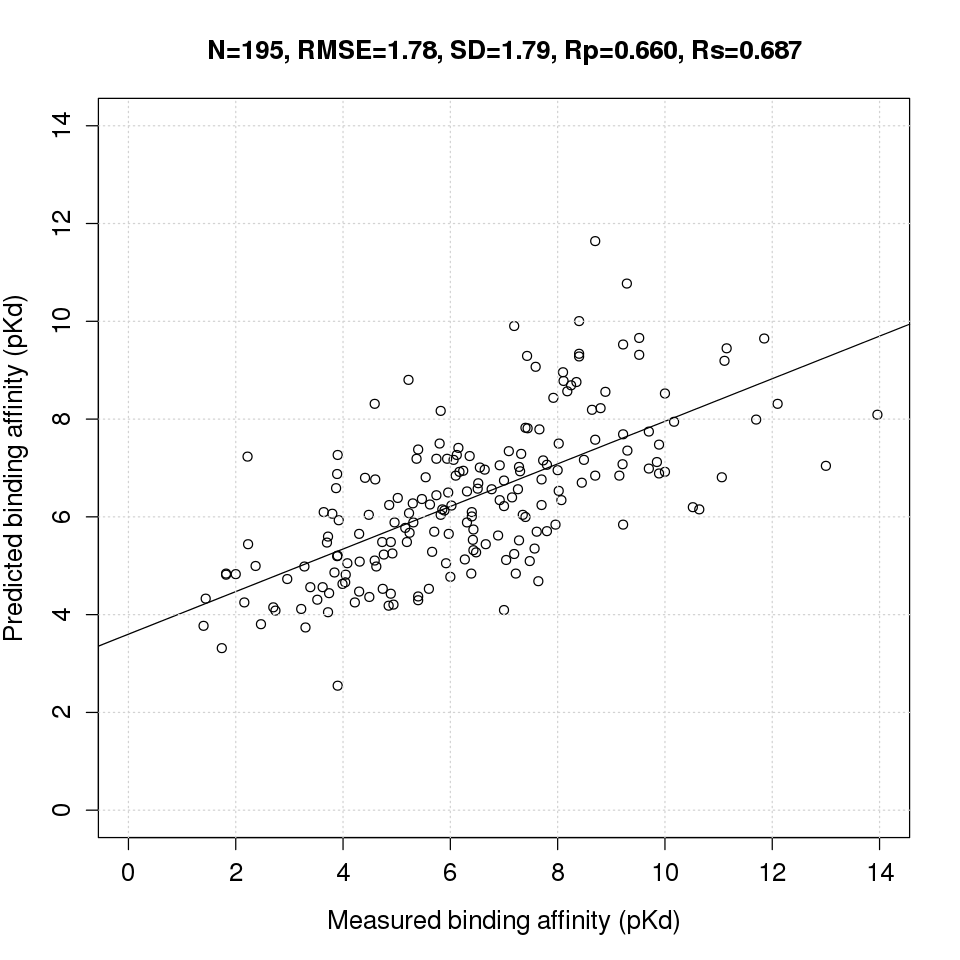
\includegraphics[width=0.8\textwidth,natwidth=960,natheight=960]{../rfcyscore/x4/mlr/trn-247-tst-195-yr.png}
  \end{center}
  \caption{An example figure}
  \label{fgr:example}
\end{figure}

\begin{table}
  \caption{Pearson's correlation coefficient $R_p$, Spearman's correlation coefficient $R_s$ and standard deviation $SD$ of the difference between predicted and experimental binding affinity on PDBbind v2007 core set ($N$ = 195). The scoring functions are sorted in the descending order of $R_p$. RF-Score, AutoDock Vina and idock rank 1st, 7th and 8th respectively in terms of Pearson's correlation coefficient $R_p$. RF-Score, ID-Score, SVR-Score and X-Score are the only scoring functions whose training set do not overlap with the PDBbind v2007 core set. The statistics for AutoDock Vina and idock are reported in this study and the statistics for the other 19 scoring functions are collected from \cite{1313,564,1305,1295}.}
  \label{tbl:example}
  \begin{tabular}{lrrr}
    \hline
Scoring function & $R_p$ & $R_s$ & $SD$\\
\hline
RF-Score & 0.774 & 0.762 & 1.59\\
ID-Score & 0.753 & 0.779 & 1.63\\
SVR-Score & 0.726 & 0.739 & 1.70\\
X-Score::HMScore & 0.644 & 0.705 & 1.83\\
DrugScoreCSD & 0.569 & 0.627 & 1.96\\
SYBYL::ChemScore & 0.555 & 0.585 & 1.98\\
AutoDock Vina & 0.554 & 0.608 & 1.98\\
idock & 0.546 & 0.612 & 1.99\\
DS::PLP1 & 0.545 & 0.588 & 2.00\\
GOLD::ASP & 0.534 & 0.577 & 2.02\\
SYBYL::G-Score & 0.492 & 0.536 & 2.08\\
DS::LUDI3 & 0.487 & 0.478 & 2.09\\
DS::LigScore2 & 0.464 & 0.507 & 2.12\\
GlideScore-XP & 0.457 & 0.435 & 2.14\\
DS::PMF & 0.445 & 0.448 & 2.14\\
GOLD::ChemScore & 0.441 & 0.452 & 2.15\\
SYBYL::D-Score & 0.392 & 0.447 & 2.19\\
DS::Jain & 0.316 & 0.346 & 2.24\\
GOLD::GoldScore & 0.295 & 0.322 & 2.29\\
SYBYL::PMF-Score & 0.268 & 0.273 & 2.29\\
SYBYL::F-Score & 0.216 & 0.243 & 2.35\\
    \hline
  \end{tabular}
\end{table}

16 classical SFs on core07 \cite{1313}

\subsection{Cyscore feature usefulness}

Compare x42 and x46

\section{Conclusions}



%%%%%%%%%%%%%%%%%%%%%%%%%%%%%%%%%%%%%%%%%%%%%%%%%%%%%%%%%%%%%%%%%%%%%
%% The "Acknowledgement" section can be given in all manuscript
%% classes.  This should be given within the "acknowledgement"
%% environment, which will make the correct section or running title.
%%%%%%%%%%%%%%%%%%%%%%%%%%%%%%%%%%%%%%%%%%%%%%%%%%%%%%%%%%%%%%%%%%%%%
\begin{acknowledgement}

We gratefully acknowledge the Direct Grant from the Chinese University of Hong Kong and the GRF Grant (Project No. 2150764) from the Research Grants Council of Hong Kong SAR, China. We also thank Yang Cao for verifying our intermediate results.

\end{acknowledgement}

%%%%%%%%%%%%%%%%%%%%%%%%%%%%%%%%%%%%%%%%%%%%%%%%%%%%%%%%%%%%%%%%%%%%%
%% The same is true for Supporting Information, which should use the
%% suppinfo environment.
%%%%%%%%%%%%%%%%%%%%%%%%%%%%%%%%%%%%%%%%%%%%%%%%%%%%%%%%%%%%%%%%%%%%%
\begin{suppinfo}



\end{suppinfo}

%%%%%%%%%%%%%%%%%%%%%%%%%%%%%%%%%%%%%%%%%%%%%%%%%%%%%%%%%%%%%%%%%%%%%
%% The appropriate \bibliography command should be placed here.
%% Notice that the class file automatically sets \bibliographystyle
%% and also names the section correctly.
%%%%%%%%%%%%%%%%%%%%%%%%%%%%%%%%%%%%%%%%%%%%%%%%%%%%%%%%%%%%%%%%%%%%%
\bibliography{../refworks}

\end{document}
